\documentclass[tikz]{standalone}
\usepackage{pgfplots}
\pgfplotsset{compat=1.15}
\usepackage{mathrsfs}
\usetikzlibrary{arrows,calc}
\usepackage{tkz-euclide}
\pagestyle{empty}

\definecolor{AngleClr}{rgb}{0,0.39215686274509803,0}
\definecolor{ShapeClr}{rgb}{0.6,0.2,0}
\definecolor{GrayClr}{RGB}{186,186,186}
\definecolor{YellowClr}{RGB}{250, 248, 217}
\definecolor{BorderClr}{RGB}{214, 190, 81}

\begin{document}

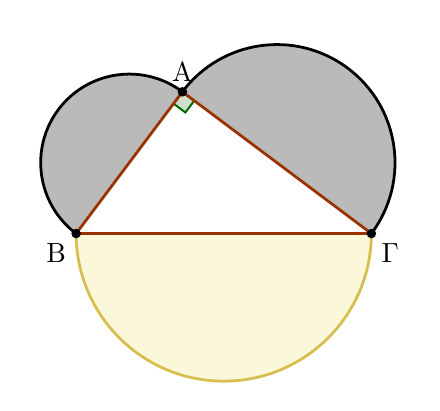
\begin{tikzpicture}[scale=.75]
\tkzSetUpLine[line width=1pt,color=black]
\tkzSetUpPoint[fill=black]

\tkzDefPoints{0/0/B,1.8/2.4/A,5/0/C}

\tkzDefCircle[circum](A,B,C) \tkzGetPoint{O}

\tkzDefMidPoint(A,B)\tkzGetPoint{MC}
\tkzDefMidPoint(B,C)\tkzGetPoint{MA}
\tkzDefMidPoint(C,A)\tkzGetPoint{MB}

\tkzDrawArc[line width=1.0pt, draw=black,fill=GrayClr](MB,C)(A)
\tkzDrawArc[line width=1.0pt, draw=black,fill=GrayClr](MC,A)(B)
% \tkzDrawCircle[line width=1.0pt, draw=black,fill=white](MA,B)
\tkzDrawArc[line width=1.0pt, draw=BorderClr,fill=YellowClr](MA,B)(C)


\tkzMarkRightAngles[line width=0.7pt, size=.25,color=AngleClr,fill=AngleClr,fill opacity=0.2](C,A,B)

\tkzDrawPolygon[color=ShapeClr](A,B,C)
\tkzDrawPoints[size=3](A,B,C)
\tkzLabelPoint[above](A){$\rm A$}
\tkzLabelPoint[below left](B){$\rm B$}
\tkzLabelPoint[below right](C){$\rm \Gamma$}

\end{tikzpicture}

\end{document}
